\documentclass[ngerman, a4paper, footsepline, headsepline]{scrreport}
\usepackage[T1]{fontenc}
\usepackage[utf8]{inputenc}
\usepackage[ngerman]{babel}
\usepackage{lmodern}
\usepackage{mathtools, amsfonts, amssymb}
\usepackage{graphicx}
\usepackage{tikz}
\usepackage{algorithm}
\usepackage{algpseudocode}
\usepackage[bottom=3.4cm, top=3cm]{geometry}
\usepackage{varioref}
\usepackage{hyperref}
\usepackage{cleveref}
\usepackage{scrlayer-scrpage}
\usepackage{siunitx}
\usepackage{enumitem}
\usepackage{xcolor}
\usepackage{listings}
\usepackage[babel]{csquotes}
\usepackage{tikzsymbols}
\usepackage{float}
\usetikzlibrary{tikzlings}
\usetikzlibrary{patterns, positioning, shapes.geometric, shapes.callouts, arrows.meta}
\usepackage[backend=biber, style=ieee]{biblatex}

%Crib pos
\definecolor{DarkGreen}{RGB}{0,100,0}

%tikz graphic
\definecolor{msg-red}{rgb}{1, 0.7, 0.56}

%lstlisting
\definecolor{main-color}{rgb}{0.6627, 0.7176, 0.7764}
\definecolor{back-color}{rgb}{0.94,0.94,0.94}
\definecolor{string-color}{rgb}{0.3333, 0.5254, 0.345}
\definecolor{key-color}{rgb}{0.13,0.13,1}
\definecolor{typedef-color}{rgb}{0.8, 0.47, 0.196}

\lstdefinestyle{mystyle}
{
	language = C,
	basicstyle = {\ttfamily\small},
	backgroundcolor = {\color{back-color}},
	stringstyle = {\color{string-color}},
	keywordstyle = {\color{key-color}},
	keywordstyle = [3]{\color{typedef-color}},
	keywordstyle = [4]{\color{teal}},
	morekeywords = [3]{uint8_t, uint32_t, bool},
	morekeywords = {restrict},
	breaklines = true,
	showstringspaces = false,
	tabsize = 4
}

\renewcommand{\lstlistingname}{Quelltext}

%\setlength{\topmargin}{-40pt} 

\newlength{\ChapterRuleWidth}\setlength{\ChapterRuleWidth}{.5pt}
\newcommand*{\ChRuleWidth}[1]{\setlength{\ChapterRuleWidth}{\dimexpr #1}}%
\newcommand*{\ChNameVar}{\setkomafont{chapterprefix}}%
\newcommand*{\ChTitleVar}{\setkomafont{chapter}}%
\newcommand*{\ChNumVar}{\setkomafont{chapternumber}}%
\newcommand*{\ChapterNameCase}[1]{#1}
\newcommand*{\ChNameUpperCase}{\let\ChapterNameCase\MakeUppercase}
\newcommand*{\ChNameIs}{\renewcommand*\ChapterNameCase[1]{##1}}
\newcommand*{\ChNameLowerCase}{\let\ChapterNameCase\MakeLowercase}
\newcommand*{\ChapterTitleCase}[1]{#1}
\newcommand*{\ChTitleUpperCase}{\let\ChapterTitleCase\MakeUppercase}
\newcommand*{\ChTitleIs}{\renewcommand*\ChapterTitleCase[1]{##1}}
\newcommand*{\ChTitleLowerCase}{\let\ChapterTitleCase\MakeLowercase}

\KOMAoptions{chapterprefix}
\ChNameUpperCase
\newkomafont{chapternumber}{\Huge}
\let\raggedchapter\raggedleft
\RedeclareSectionCommand[%
beforeskip=-5pt,
innerskip=45pt,
afterskip=40pt,
font=\normalfont\sffamily\Large,
prefixfont=\Large,
]{chapter}
\renewcommand*{\chapterformat}{%
	\mbox{\ChapterNameCase{\chapappifchapterprefix{\nobreakspace}}%
		{\usekomafont{chapternumber}{%
				\rule{0pt}{.8\baselineskip}\thechapter\IfUsePrefixLine{}{\enskip}}}%
	}%
}
\renewcommand*{\chapterlineswithprefixformat}[3]{% 
	\IfArgIsEmpty{#2}{}{%
		#2%
	}%
	\rule[5pt]{\linewidth}{\ChapterRuleWidth}\\*
	\ChapterTitleCase{#3}\nobreak
	\rule[-5pt]{\linewidth}{\ChapterRuleWidth}
}

\newcommand{\fmbox}[1]{
	\begin{center}
		\fcolorbox{black}{yellow}
		{\parbox{0.88\textwidth}
			{\textcolor{black}
				{#1}
			}
		}
	\end{center}
}

\definecolor{func-red}{rgb}{1, 0.7, 0.56}

\newcommand{\scalepic}{.8}

\pagestyle{scrheadings}
\newcommand{\myifoot}{\textbf{Emanuel Schäffer}}
%\newcommand{\mycfoot}{\textbf{RWU--University of Applied Sciences}}
\automark{section}
%\ofoot{\mycfoot}
\ohead{\headmark}
\chead{}
\ifoot{\myifoot}

\sisetup{
	locale=DE,
	group-separator= {\,}
}




\addbibresource{sources.bib}
\addbibresource{pictures.bib}

\MakeOuterQuote{"}

\begin{document}
	\subject{Kryptoanalyse der Enigma-Maschine durch eine Software-Nachbildung der Turing-Welchman-Bombe}
	\title{Turing-Welchman-Bombe}
%	\titlehead{}
	\author{Emanuel Schäffer}
	\date{\today}
	\publishers{RWU--University of Applied Sciences \\ Prof. Dipl.-Math. Ekkehard Löhmann}
	\maketitle
	
	\tableofcontents
	
	\chapter{Einleitung}\label{ch:einleitung}
	Diese Projektarbeit beschäftigt sich mit der Kryptoanalyse der Enigma-Maschine.
	Im Speziellen wird hier auf die Kryptoanalyse mit der von Alan Turing und Gordon Welchman entwickelten \glqq Turing-Welchman-Bombe\grqq{} eingegangen.
	Die Turing-Welchman-Bombe baut auf die Arbeit von Marian Rejewski und seiner \glqq Bomba\grqq{} auf, welche der Turing-Welchman-Bombe ihren Namen gab.
	Dieses Verfahren zur Kryptoanalyse spielte eine wesentliche Rolle im Zweiten Weltkrieg und trug nach der Meinung vieler Historiker maßgeblich dazu bei, den Krieg zu verkürzen und rettete somit zahlreiche Menschenleben.
	% 2 Jahre 14 Mio. Menschenleben
	
	
	\documentclass[ngerman, a4paper, footsepline, headsepline]{scrreport}
\usepackage[T1]{fontenc}
\usepackage[utf8]{inputenc}
\usepackage{babel, lmodern, scrlayer-scrpage, amsmath, amsmath, amsfonts, graphicx, tikz, algorithm, algpseudocode}
\usepackage[bottom=4cm]{geometry}

\pagestyle{scrheadings}
\newcommand{\myifoot}{\textbf{Emanuel Schäffer}}
%\newcommand{\mycfoot}{\textbf{RWU--University of Applied Sciences}}
\automark{section}
%\ofoot{\mycfoot}
\ohead{\headmark}
\chead{}
\ifoot{\myifoot}

\newcommand{\figref}[1]{(siehe Abb.~\ref{#1})}

\newcommand{\aszboxy}[1]{
	\begin{center}
		\fcolorbox{black}{yellow}
		{\parbox{0.88\textwidth}
			{\textcolor{black}
				{#1}
			}
		}
	\end{center}
}

\begin{document}
	\subject{Kryptoanalyse der Enigma-Maschine: Eine Untersuchung des Cyclometers und der Turing-Bombe}
	\title{Kryptoanalyse der Enigma-Maschine}
	\author{Emanuel Schäffer}
	\date{\today}
	\publishers{RWU--University of Applied Sciences}
	\maketitle
	
	\begin{abstract}
		Enigma-Nachrichten können dechiffriert werden, wenn die Rotorauswahl, die Rotor-~, Ringstellungen und die Steckereinstellungen einzeln wiederhergestellt werden. Die Wiederherstellung der Nachrichtenschlüsseleinstellung ist empfindlich genug, um die korrekte Rotorreihenfolge zu unterscheiden. 
	\end{abstract}


	\chapter{Enigma}
	\section{Einführung}
	Die Enigma ist eine Rotor-Chiffriermaschine, die hauptsächlich im Zweiten Weltkrieg Einsatz kam. Die von der Wehrmacht modifizierte Enigma verfügte zunächst über drei Walzen und zusätzlich einen Reflektor. Jede dieser Walzen führte eine monoalphabetische Substitution durch. Die rechte Walze wurde bei jedem Tastendruck um eine Position weitergerückt. Hat diese Walze eine komplette Rotation vollzogen, rückte die Walze links neben ihr um eine Position weiter\footnote{Eine Analogie hierfür ist der Kilometerzähler eines mechanischen Tachometers oder das Verhalten von Sekunden-, Minuten- und Studenzeigern einer Uhr.}. Neuerungen waren das Steckerbrett \figref{fig:enigma_complete} und gegen Ende des Krieges eine zusätzliche, vierte Walze. Ich werde mich, wenn nicht ausdrücklich erwähnt, auf die Enigma M3 mit drei Walzen beschränken.
	\nopagebreak
	\begin{figure}[htbp]
		\centering
		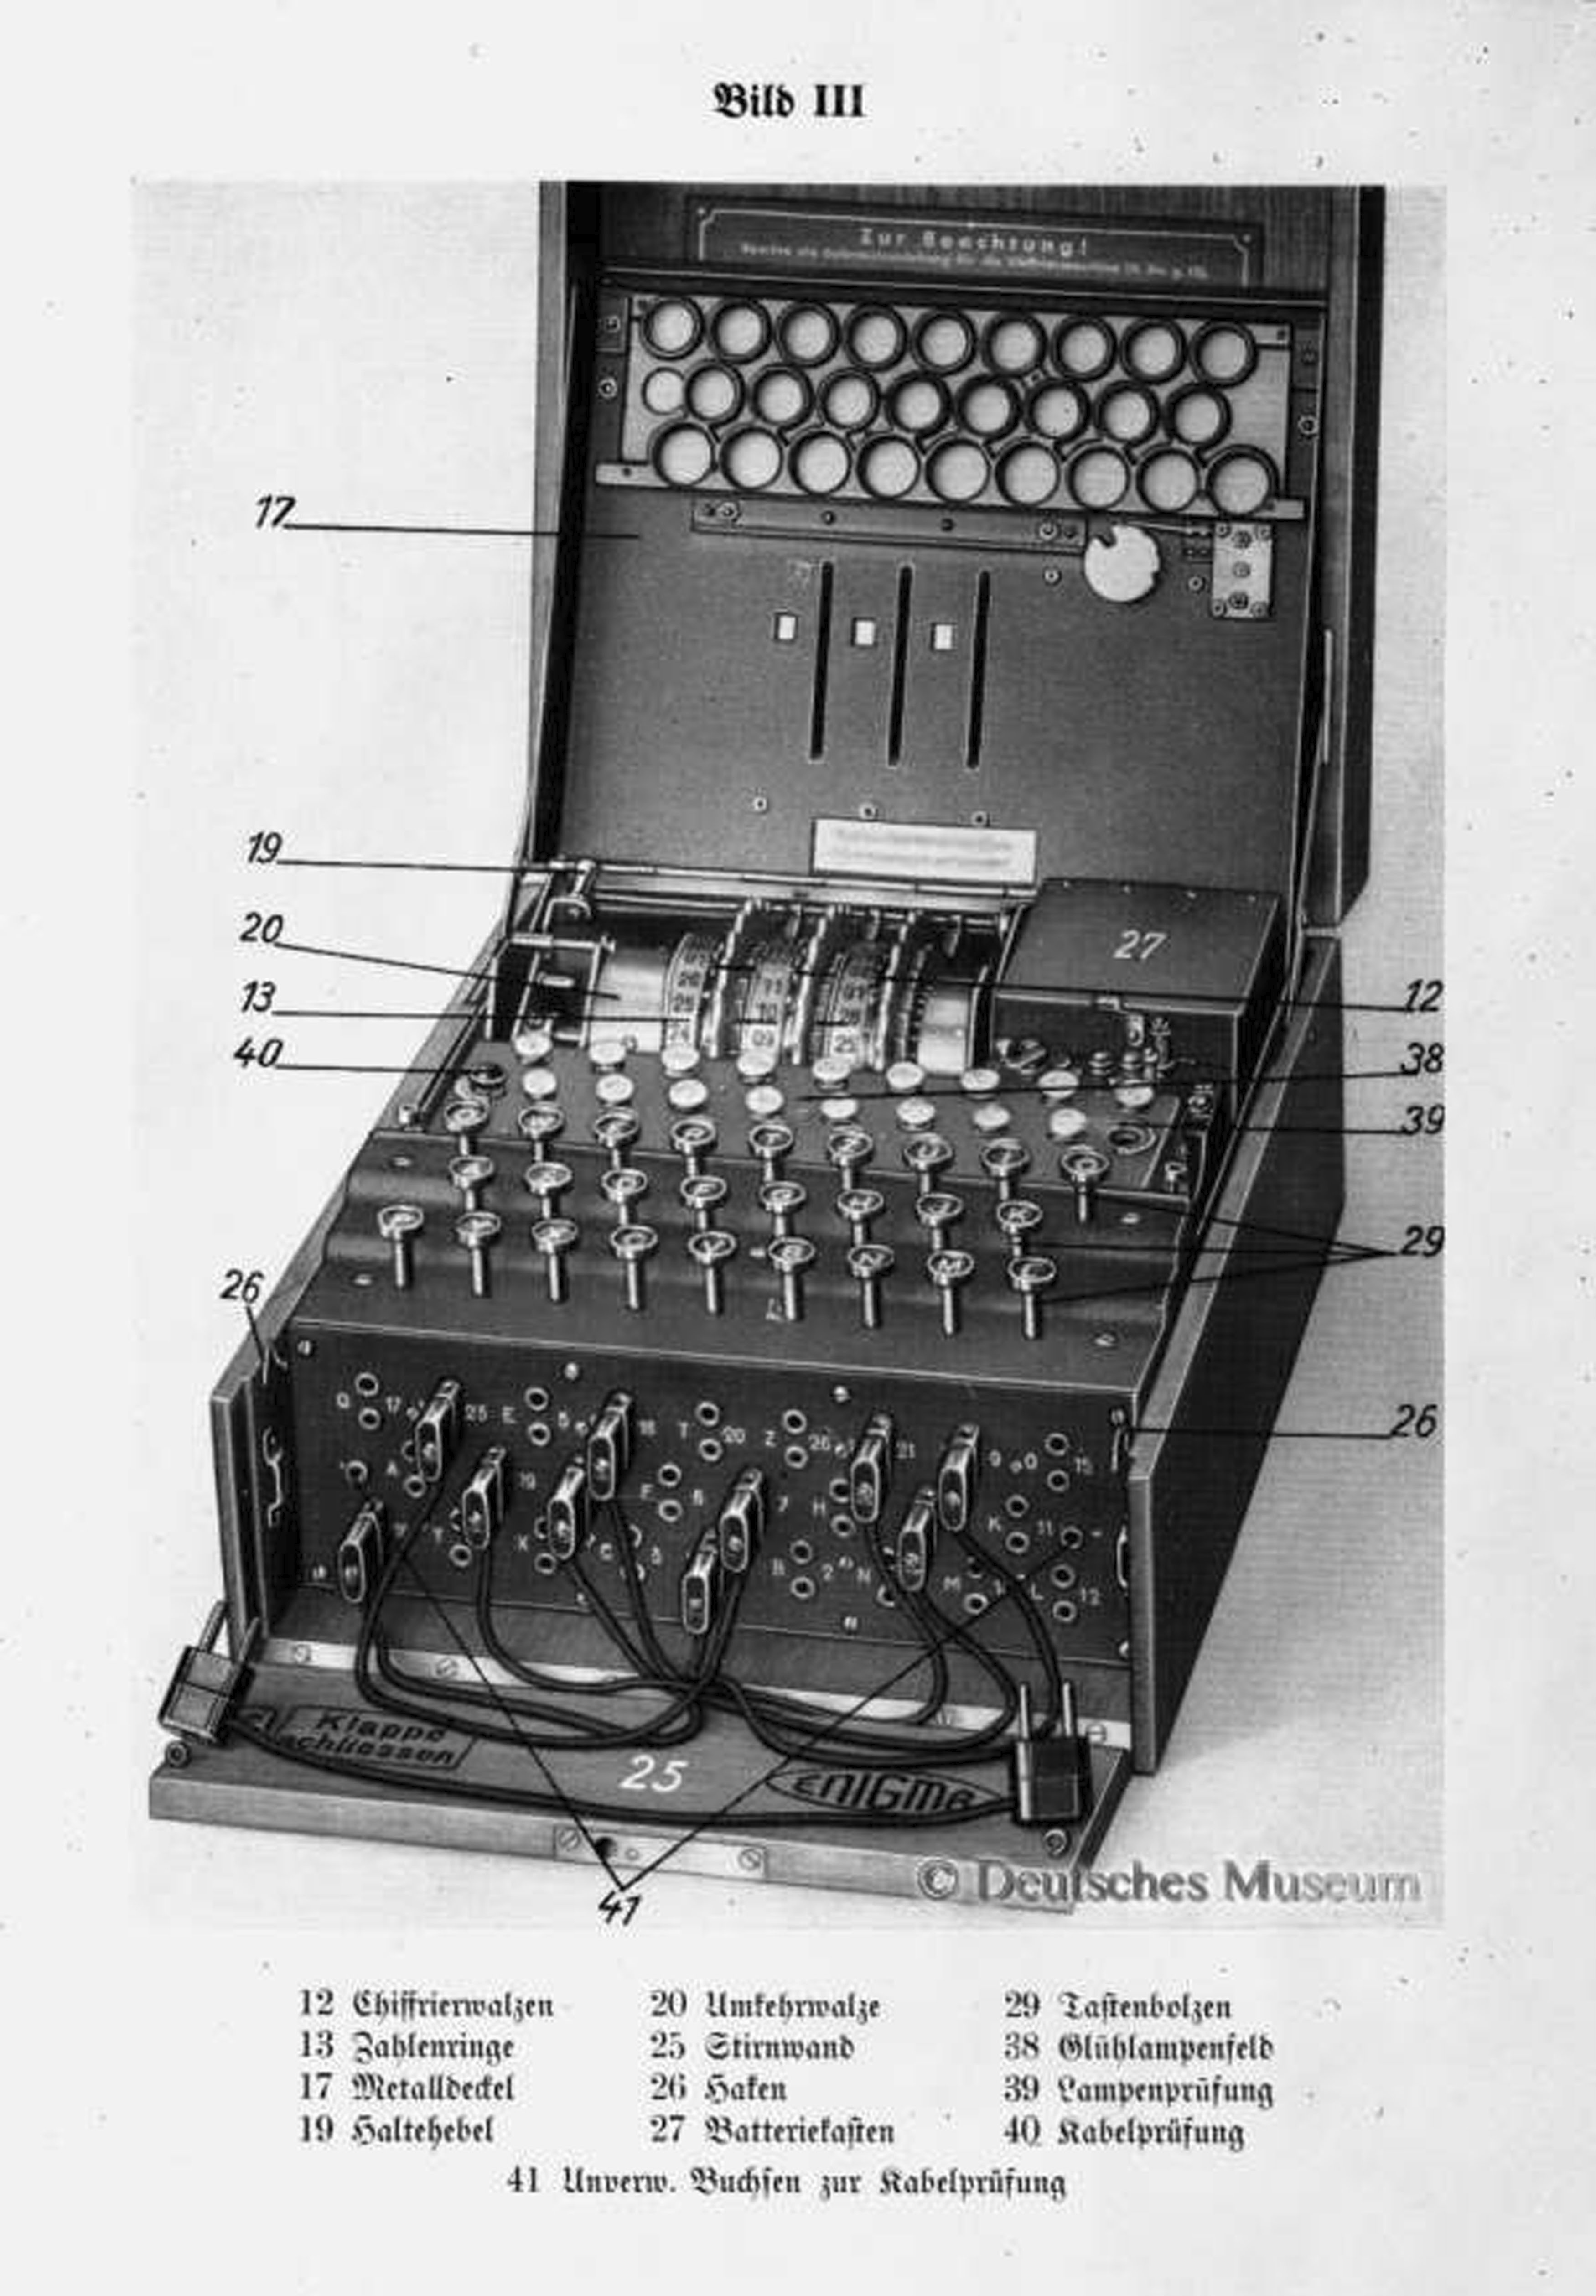
\includegraphics[width=.5\linewidth]{Enigma-komplett.png}
		\caption{Die Enigma Maschine}
		\label{fig:enigma_complete}
	\end{figure}
	
	\newpage
	
	 Bei der Enigma wurde jeden Tag  eine Tagesschlüssel eingestellt, welcher durch ein Code-Buch vorgegeben war. Dieser Tagesschlüssel bestand darin, welche drei der fünf Walzen der Schlüssler in welcher Reihenfolge einzusetzen hatte. Ferner musste er die Walzenstellung einstellen. Sie bestimmt die Ausgangsstellung der Walzen. Diese konnte durch ein Sichtfenster abgelesen werden.
	
	\begin{figure}[htbp]
		\centering
		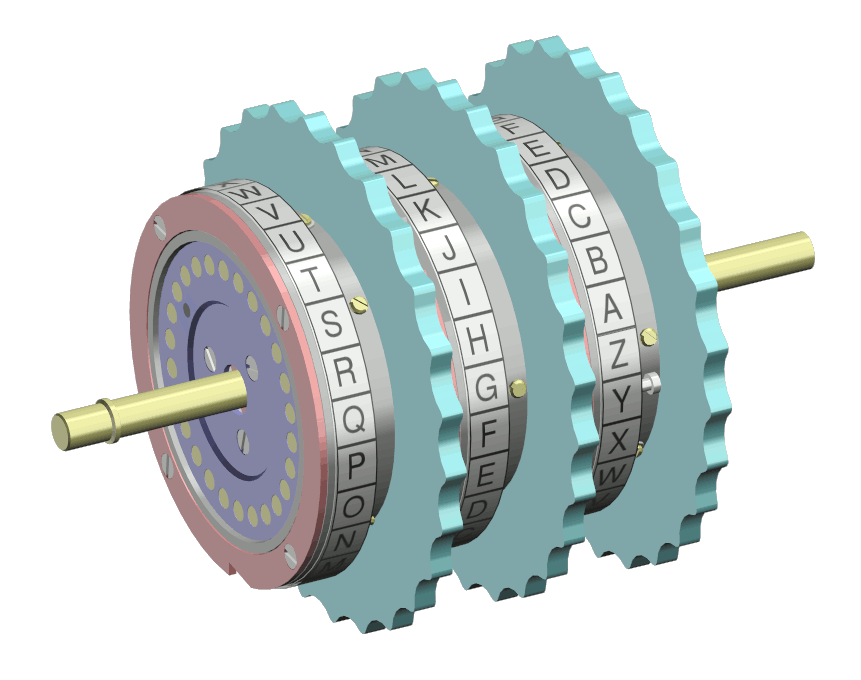
\includegraphics[width=.4\linewidth]{Enigma-rotor-set.png}
		\caption{Enigma-Walzen}
		\label{fig:enigma_rotors}
	\end{figure}
	
	Zusätzlich musste der Schlüssler die Ringstellung des Tages einstellen. Die Ringstellung veränderte die Relation der sichtbaren Buchstaben mit der internen Verdrahtung und bewegte die Übertragskerbe \figref{fig:enigma-rotor-contact}, die festlegte, wann sich die Walze links von der aktuellen bewegt.
	
	\begin{figure}[htbp]
		\centering
		\begin{tikzpicture}
			\node at (0,0) {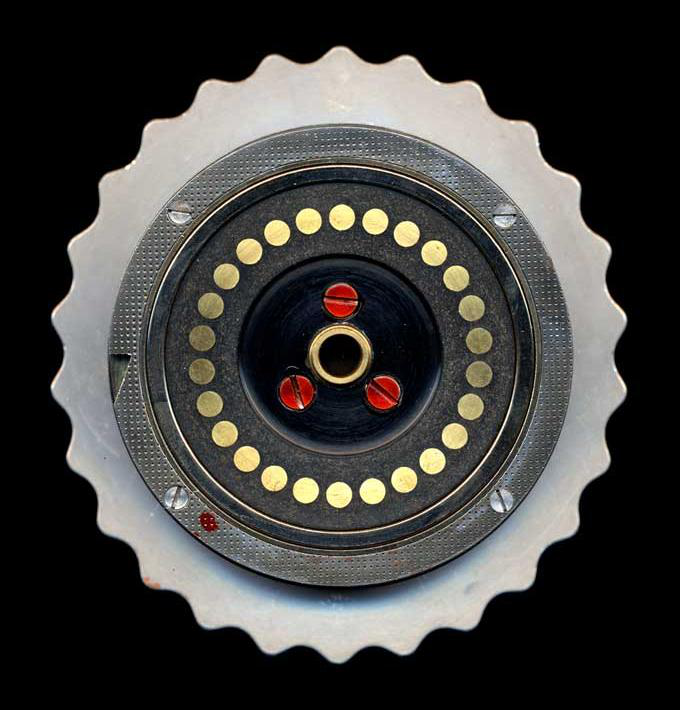
\includegraphics[width=.3\linewidth]{Enigma-rotor-flat-contacts.png}};
			\draw[red, very thick, ->] (-3,-0.5) -- (-1.5,-0.1) ;
			\node[red, anchor=west] at (-5,-0.8) {Übertragskerbe};
		\end{tikzpicture}
		\caption{Walzen Frontansicht mit Übertragskerbe}
		\label{fig:enigma-rotor-contact}
	\end{figure}
	
	\newpage
	Als letzte Einstellung musste das Steckerbrett verdrahtet werden. Das Steckerbrett vertauschte zwei Buchstaben miteinander. Von 13 möglichen Steckerverbindungen wurden meistens 10 vorgegeben. 
		
		
	Wenn der Schlüssler nun eine Taste auf der Tastatur betätigte, floss Strom durch das Steckerbrett, welches eine Substitution durchführt. Danach floss der Strom durch den Walzensatz, in den Reflektor und nochmals in entgegengesetzter Richtung durch den Walzensatz. Jeder dieser Walzen führte eine monoalphabetische Substitution durch. Nach dem der Strom den Walzensatz verlassen hatte, floss der Strom nochmals durch das Steckerbrett und erleuchtete letztendlich eine Lampe.
	\begin{figure}[htbp]
		\centering
		\caption{Verdrahtung Walze I}
		\resizebox{\textwidth}{!}{%
			\begin{tabular}{|c|c|c|c|c|c|c|c|c|c|c|c|c|c|c|c|c|c|c|c|c|c|c|c|c|c|}
				\hline	
				A & B & C & D & E & F & G & H & I & J & K & L & M & N & O & P & Q & R & S & T & U & V & W & X & Y & Z\\
				\hline
				E & K & M & F & L & G & D & Q & V & Z & N & T & O & W & Y & H & X & U & S & P & A & I & B & R & C & J\\
				\hline
			\end{tabular}
		}
		\label{fig:rot1_cabeling}
	\end{figure}
	
	
	
	
	\section{Übertragung der Nachrichten}
	Nachdem alle Einstellung getroffen waren, überlegte sich der Schlüssler einen "`zufälligen"' Spruchschlüssel, mit dem der Text verschlüsselt wurde.\footnote{In Wahrheit wählten die Schlüssler oft den gleichen Schlüssel, der meist persönliche Informationen wie zum Beispiel den Name der Freundin enthielt.} Dieser Spruchschlüssel gab die Walzenstellung für die folgende Nachricht an. Der "`zufällige"' Spruchschlüssel wurde mit dem Tagesschlüssel verschlüsselt und ergab zusammen mit anderen Zusatzinformationen den "`Spruchkopf"'. Der Schlüssler gab nun den zu verschlüsselnden Text nach bestimmten Regeln ein. Eine Eigenschaft der Enigma ist, dass sie selbstinvers ist. Das bedeutet, dass mit der gleichen Einstellung, mit der ein Text verschlüsselt wurde, dieser auch wieder entschlüsselt werden kann.
	
	
	
	
	\chapter {Bombe}
	
	\section{Algorithmus Bombe}
	
	\begin{algorithm}
		\caption{Bombe Algorithmus}
		\begin{algorithmic}[1]
			\Procedure{Bombe}{$p_0 \dots p_{n-1} :$ [Char], $c_0 \dots c_{n-1} :$ [Char]}
				\ForAll{\textsl{rotors} $\in$ \textbf{permut(rotor order)}, \textsl{pos} $\in$ \textbf{[AAA $\dots$ ZZZ]}}
					\State plugs: Char $\rightarrow \{ $Char$\}$
					\State plugs$(p_0)\ \cup= \{\textbf{'A'}\}$
					\While{\textsl{plugs} changing}
						\ForAll{\textsl{i} $\in$ \textbf{[0\dots n--1]}}
							\State plugs($c_i$) $\cup=$ $\bigcup_{p \in \text{plugs}(p_i)}$ encrypt(\textsl{rotors, p, pos}+\textsl{i})
							\State plugs($p_i$) $\cup=$ $\bigcup_{p \in \text{plugs}(c_i)}$ encrypt(\textsl{rotors, p, pos}+\textsl{i})
						\EndFor
					\EndWhile
					\If{$\forall$ \textsl{S} $\in$ \textbf{cod(plugs)}: \#S < \#Char}
						\State report(\textsl{pos, plugs})
					\EndIf
				\EndFor
			\EndProcedure
		\end{algorithmic}
	\end{algorithm}
	
	\section{Cycle Finding Algorithm}
	\noindent
	\texttt{typedef struct \{} \\
	\hspace*{0.5cm} \texttt{char first;} \\
	\hspace*{0.5cm} \texttt{char second;} \\
	\texttt{\} Tuple;}
		\begin{algorithm}
			\caption{Cycle Finding Algorithm}
			\begin{algorithmic}[1]
				\Procedure{is\_cyle}{$start :$ \textbf{char}, $c:$ char, $tuples_0 \dots tuples_{n-1}:$ Tuple, $visited\_mask:$ uint32\_t}
				\EndProcedure
			\end{algorithmic}
		\end{algorithm}
	
	
	
	\chapter{Häufigkeitsanalyse}
	\section{Koinzidenzindex}
	\thispagestyle{scrheadings}
	
	Zunächst benötigen wir ein geeignetes Maß, um den Grad der Annäherung eines teilweise dechiffrierten Klartextes an authentisches Deutsch abzuschätzen. Dafür verwenden wir den Koinzidenzindex:
	
	$$
	IC = \frac{\sum_{i=A}^{Z}f_i(f_i-1)}{N(N-1)}
	$$
	
	Sei $f_i$ die Häufigkeit des Buchstabens in Abhängigkeit von $i$ und $N$ die Gesamtanzahl der Buchstaben. Wir Summieren also die Anzahl der Buchstabenpaare auf, und teilen diese durch die Anzahl der allgemein möglichen Buchstabenpaare. Der Koinzidenzindex ist also ein Maß für die Buchstabenverteilung. Für ein Text bestehend aus zufälligen Buchstaben beträgt der $IC \approx$ 0.038; wobei er für Deutsch $\approx$ 0.076 beträgt.
	\newpage
	
	Bemerkungen:
	
	Improvements:
	
	Base: 8.5s
	
	Nur letzte Buchstaben testen: 3.6s
	
	IC: 3.3s
	
	Low Level IO: 3.31s
	
	Nur erster char testen an der Position, an dem das Schlagwort stehen muss: 2.25s 
	
	
	\chapter{Quellen}
	
	%Deutsches Museum, Ertl Angewandte Kryptographie \ref{fig:enigma_complete}
	
	%https://upload.wikimedia.org/wikipedia/commons/9/9f/Enigma_rotor_set.png Zugriff %11.09.24. 10:57 \ref{fig:enigma_rotors}
	
	%https://de.wikipedia.org/wiki/Enigma-Walzen#/media/Datei:Enigma-rotor-flat-contacts.jpg Zugriff 11.09.24. 11:19 \ref{fig:enigma-rotor-contact}
	
	
	
\end{document}
	
	\chapter{Die Turing-Welchman-Bombe}\label{ch:die-turing-bombe}

\section{Einführung}\label{sec:einfuerung_bombe}

Da frühe Verfahren zur Kryptoanalyse der Enigma-Maschine, wie zum Beispiel der \glqq Zyklometer\grqq{} oder die \glqq Bomba\grqq{}, durch die Einführung einer neuen Umkehrwalze (UKW-B), neuen Walzen und Änderung des Schlüsselverfahrens unbrauchbar gemacht wurden, musste ein neues Verfahren zur Kryptoanalyse der Enigma-Maschine von den Alliierten entwickelt werden. 
Der Durchbruch gelang, wie auch schon bei Marian Rejewski und seiner Bomba und Zyklometer, einem, beziehungsweise zwei Mathematikern.
Alan Turing und Gordon Welchman waren die Hauptverantwortlichen für die Entwicklung der \glqq Turing-Welchman-Bombe\grqq.
Dieses Verfahren basiert ähnlich wie der Zyklometer auf \glqq Zyklen\grqq.
Jedoch wurde hier nicht die Verdopplung des Spruchschlüssels im Spruchkopf ausgenutzt, sondern Zyklen zwischen einem an einer bestimmten Stelle im Geheimtext vermuteten Klartext (Crib) und dem Geheimtext bestimmt.
Die Turing-Welchman-Bombe testet immer eine Hypothese einer Steckerbrett-Verbindung und probierte mit drei von acht möglichen Walzen alle Walzenstellungen durch.
Auch wenn diese Hypothese sich als nicht korrekt erwies, findet die Turing-Welchman-Bombe bei korrekter Walzenlage durch Reductio ad absurdum trotzdem die gültigen Steckerbrett-Verbindungen.
Ziel war es, die abgefangene Nachricht und ultimativ den Tagesschlüssel zu knacken.
Aufgrund der Einfachheit wird im Folgenden der Begriff \glqq Bombe\grqq{} anstelle von \glqq Turing-Welchman-Bombe\grqq{} verwendet.
\vspace{-13pt}
\begin{figure}[H]
	\centering
	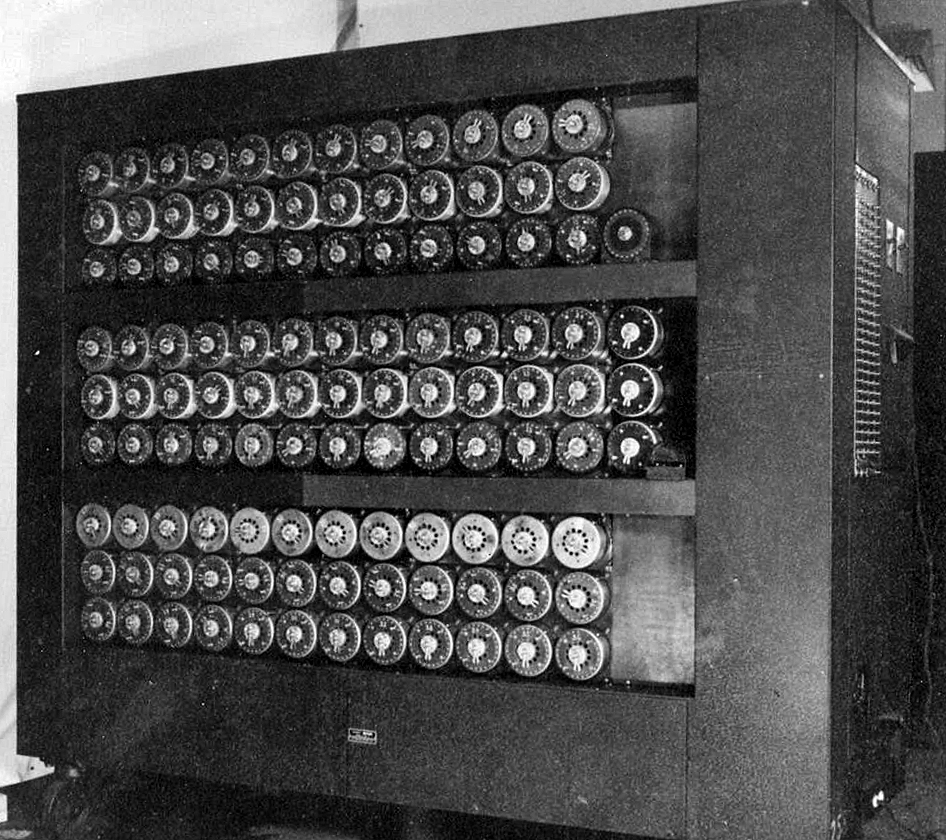
\includegraphics[width=0.39\linewidth]{Turing Bomb/BletchleyParkBombe}
	\caption{Eine Turing-Welchman-Bombe in Bletchley Park\autocite{wiki:bombe_picture}}
	\label{fig:bombe}
\end{figure}
\vspace{-2em}

\section{Funktionsweise}\label{sec:funktionsweise_bombe}

\subsection{Vorbereitungen}\label{subsec:vorbereitungen}

\subsubsection{Crib}\label{subsubsec:crib}
Hier wird der Anglizismus \glqq Crib\grqq{} verwendet, da dieser Begriff keine richtige Deutsche Übersetzung hat.

Ein Crib ist ein Klartextfragment, welches an einer bestimmten Stelle im Geheimtext vermutet wird. 
Die deutsche Wehrmacht verwendete in den gesendeten Nachrichten häufig Floskeln. 
Ein Beispiel hierfür ist: \glqq Das Oberkommando der Wehrmacht gibt bekannt\grqq.
Nun musste das Crib positioniert werden.
Wie in~\cref{subsec:umkehrwalze} erklärt, ist es nicht möglich, dass ein Buchstabe auf sich selbst abgebildet wird.
Wurde eine mögliche Position gefunden, konnten die Mitarbeiter von Bletchley Park anfangen, das sogenannte Menü zu bauen.
Die~\cref{fig:positioning_crib} zeigt solch eine Positionierung.

\begin{figure}[htbp]
	\centering
	\caption{Positionierung des Cribs}
	\label{fig:positioning_crib}
	\resizebox{\linewidth}{!}{
		\ttfamily
		\begin{tabular}{|c|c|c|c|c|c|c|c|c|c|c|c|c|c|c|c|c|c|c|c|c|c|c|c|c|c|c|c|}
			\hline
			B & H & N & C & X & S & E & Q & K & O & B & I & I & O & D & W & F & B & T & Z & G & C & Y & E & H & Q & Q & J \\
			\hline
			O & B & E & R & K & O & M & M & A & N & D & O & D & E & R & \textcolor{red}{W} & E & H & R & M & A & \textcolor{red}{C} & H & T & & & &\\
			\hline
			\multicolumn{1}{|c|}{} & \textcolor{DarkGreen}{O} & \textcolor{DarkGreen}{B} & \textcolor{DarkGreen}{E} & \textcolor{DarkGreen}{R} & \textcolor{DarkGreen}{K} & \textcolor{DarkGreen}{O} & \textcolor{DarkGreen}{M} & \textcolor{DarkGreen}{M} & \textcolor{DarkGreen}{A} & \textcolor{DarkGreen}{N} & \textcolor{DarkGreen}{D} & \textcolor{DarkGreen}{O} & \textcolor{DarkGreen}{D} & \textcolor{DarkGreen}{E} & \textcolor{DarkGreen}{R} & \textcolor{DarkGreen}{W} & \textcolor{DarkGreen}{E} & \textcolor{DarkGreen}{H} & \textcolor{DarkGreen}{R} & \textcolor{DarkGreen}{M} & \textcolor{DarkGreen}{A} & \textcolor{DarkGreen}{C} & \textcolor{DarkGreen}{H} & \textcolor{DarkGreen}{T} & & & \\
			\hline
			\multicolumn{2}{|c|}{} & O & B & E & R & K & O & M & M & A & N & D & \textcolor{red}{O} & \textcolor{red}{D} & E & R & W & E & H & R & M & A & C & \textcolor{red}{H} & T & & \\
			\hline
			\multicolumn{3}{|c|}{} & \textcolor{DarkGreen}{O} & \textcolor{DarkGreen}{B} & \textcolor{DarkGreen}{E} & \textcolor{DarkGreen}{R} & \textcolor{DarkGreen}{K} & \textcolor{DarkGreen}{O} & \textcolor{DarkGreen}{M} & \textcolor{DarkGreen}{M} & \textcolor{DarkGreen}{A} & \textcolor{DarkGreen}{N} & \textcolor{DarkGreen}{D} & \textcolor{DarkGreen}{O} & \textcolor{DarkGreen}{D} & \textcolor{DarkGreen}{E} & \textcolor{DarkGreen}{R} & \textcolor{DarkGreen}{W} & \textcolor{DarkGreen}{E} & \textcolor{DarkGreen}{H} & \textcolor{DarkGreen}{R} & \textcolor{DarkGreen}{M} & \textcolor{DarkGreen}{A} & \textcolor{DarkGreen}{C} & \textcolor{DarkGreen}{H} & \textcolor{DarkGreen}{T} & \\
			\hline
			\multicolumn{4}{|c|}{} & O & B & \textcolor{red}{E} & R & \textcolor{red}{K} & \textcolor{red}{O} & M & M & A & N & \textcolor{red}{D} & O & D & E & R & W & E & H & R & M & A & C & H & T \\
			\hline
		\end{tabular}
	}
\end{figure}	

In Bletchley Park waren zudem viele Sprachexperten beschäftigt, die darauf spezialisiert waren, solche Cribs zu erstellen.
Dies erforderte sowohl sehr gute Kenntnisse über die Deutsche Sprache, als auch sehr gute Kenntnisse über die in~\cref{sec:uebertragung-der-nachrichten}
beschriebenen Regeln zu Funkspruch-Verschlüsselung.
Zudem mussten Eigenheiten und die \glqq Schreibfäule\grqq{} der Funker beachtet werden.
Ein Crib wurde unter der Vermutung benutzt, dass während der kompletten Eingabezeit des Abschnittes nur die rechte Walze (schnelle) Walze rotiert hat.
Aus diesem Grund darf ein Crib nicht länger als 25 Buchstaben sein, da sonst gewiss ein Übertrag auf die mittlere Enigma-Walze stattfand.
Die Bombe vernachlässigt also den Übertragzeitpunkt der Enigma-Walzen, wodurch die Ringstellung keine weitere Rolle spielt.
Um das Risiko zu minimieren, dass ein Übertrag stattgefunden hat, wurden meist Cribs mit einer Länge von ungefähr 13 Buchstaben verwendet.
In unserem Fall wäre also das Crib \glqq OBERKOMMANDODERWEHRMACHT\grqq{} zu lang.
Da das Crib jedoch keinen linguistischen Sinn ergeben muss, könnte man dies einfach zu \glqq OBERKOMMANDODER\grqq{} kürzen.

Eine Strategie der Alliierten für die Erzeugung von Cribs war zum Beispiel das sogenannte \glqq Gardening\grqq.
Damit ist das bewusste Provozieren von Funksprüchen, die einen bestimmten Klartext enthalten gemeint.
Eine Strategie war es, Seeminen in Flüsse, Häfen oder Seegebiete abzuwerfen.
Dafür musste ein Funker-Trupp in der Nähe des Ereignisses sein, welcher nicht verletzt werden durfte.
Ein mögliches Ziel war hier zum Beispiel ein Seegebiet in der Nähe eines U-Boots, da diese stets eine Enigma-Maschine an Bord hatten.
Nun beinhaltete der kurz darauf folgende Funkspruch mit einer hohen Sicherheit das Wort: \glqq Minen\grqq.

\subsubsection{Menü}\label{subsubsec:menu}
Nun werden Buchstaben-Tupel zwischen Crib und Geheimtext gebildet.
An einem Beispiel von \glqq WETTERVORHERSAGE\grqq{} und \glqq SNMKGGSTZZUGARLV\grqq{} wären solche Tupel: \texttt{W:S}, \texttt{E:N} et cetera.
Nun werden die Tupel mit passenden Buchstaben aneinander gesetzt. 
In dem obigen Beispiel wären die Tupel unter anderem: $\texttt{W:S} - \texttt{S:V} - \texttt{V:E}$.
Der daraus resultierende Graph wird \glqq Menü\grqq{} genannt.
Er gibt die Einstellungen der Bombe vor.
\nopagebreak
\begin{figure}[htbp]
	\centering
	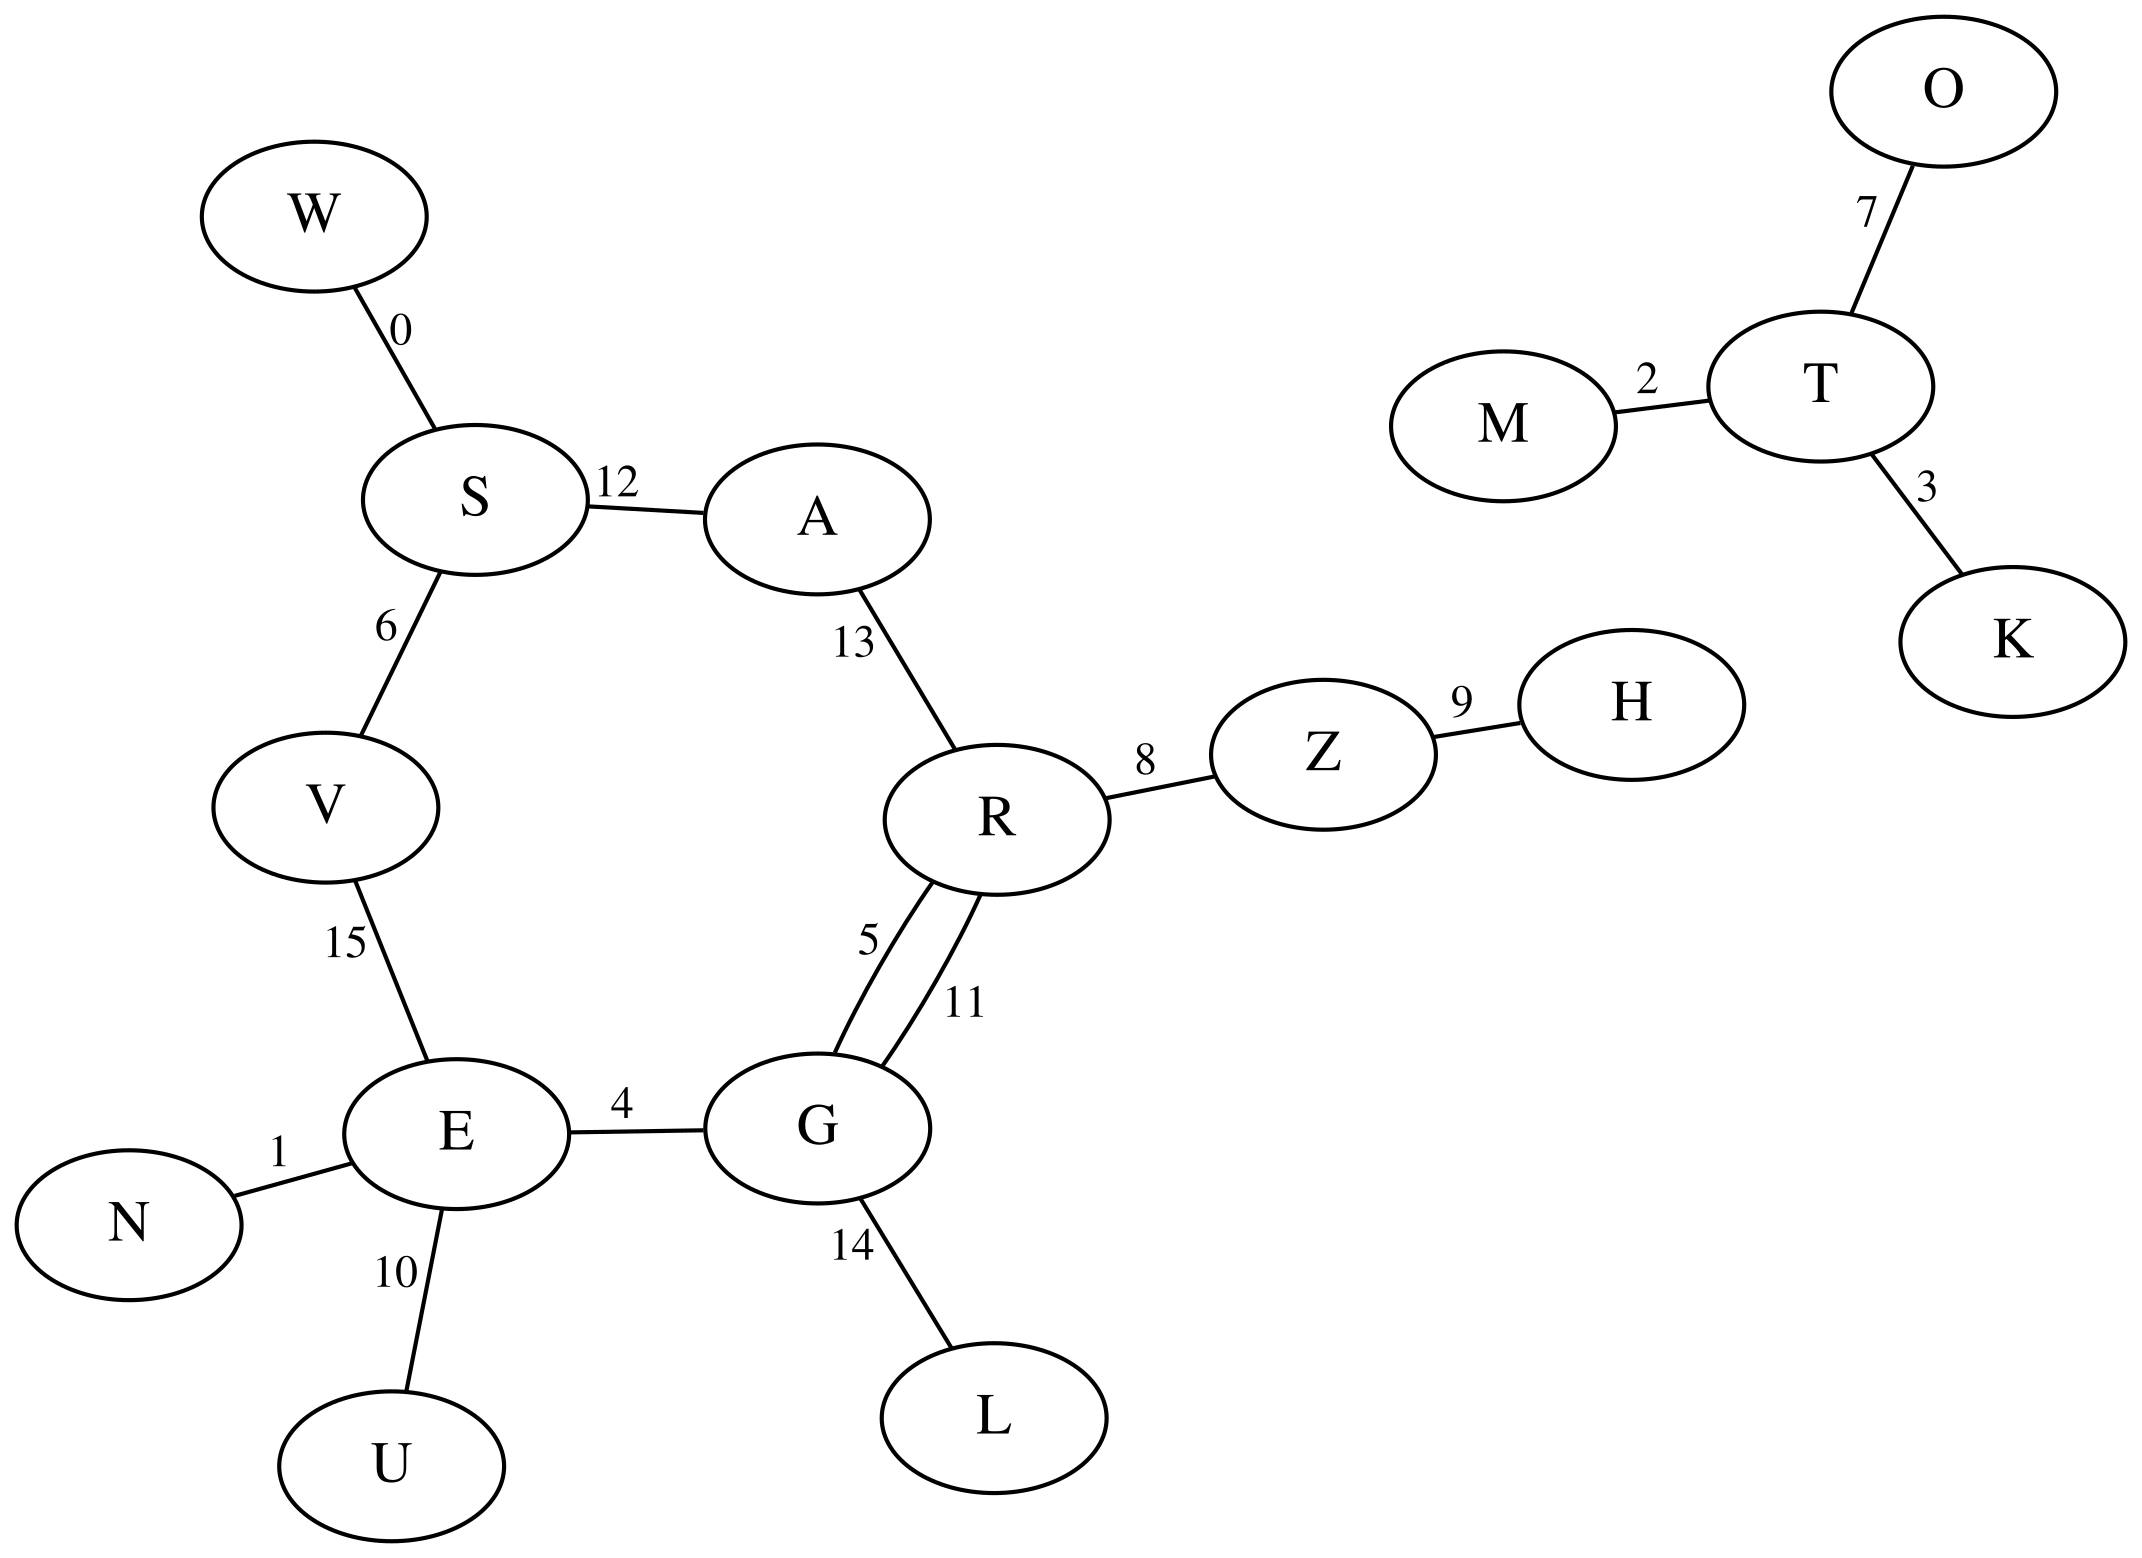
\includegraphics[width=.6\linewidth]{Turing Bomb/crib_cipher_cycle}
%	\includegraphics[width=.6\linewidth]{Turing Bomb/crib_cycle_cipher_graph}
	\caption{Crib-Geheimtext Menü}
	\label{fig:crib_cipher_cycle}
\end{figure}

Wenn sich wie in~\cref{fig:crib_cipher_cycle} ein Zyklus bildet, ist dies eine brauchbare Crib-Geheimtext-Kombination.
Alan Turing machte die Beobachtung, dass die Steckerbrett-Verbindungen der Enigma-Maschine keinen Einfluss auf den Verlauf des Menüs haben.
Dies ist durch die Eigenschaft des Steckerbrettes der Enigma-Maschine gegeben, welche eine monoalphabetische Substitution durchführt, die sich über den kompletten Chiffrierungs-Prozess nicht ändert.

Die Zahlen auf den Kanten geben hierbei die Position des Tupels innerhalb der gefundenen Crib-Geheimtext Kombination an.
Tupel wie 0, 1, 8, 9, 10 und 14 werden hier als \glqq Ausleger\grqq{} bezeichnet, da diese nicht aktiv zum Zyklus beitragen, aber trotzdem von Relevanz bei der Kryptoanalyse sind.
Aus Gründen, die später erläutert werden, sind Tupel-Kombinationen wie 5 und 11 äußerst effektiv für die Kryptoanalyse.
Tupel, die keinen Zyklus bilden, können ignoriert werden.
Somit sind die Tupel 2, 3 und 7 für den weiteren Verlauf der Kryptoanalyse irrelevant.

\subsection{Scrambler}\label{subsec:scrambler}
Wie auch die Enigma-Maschine hat auch die Bombe \glqq Walzen\grqq.
Jedoch haben diese nicht 52, sondern 104 Kontakte, da es erforderlich war, diese miteinander zu verbinden.
Die Walzen der Bombe werden oft Scrambler genannt.

\begin{figure}[htbp]
	\centering
	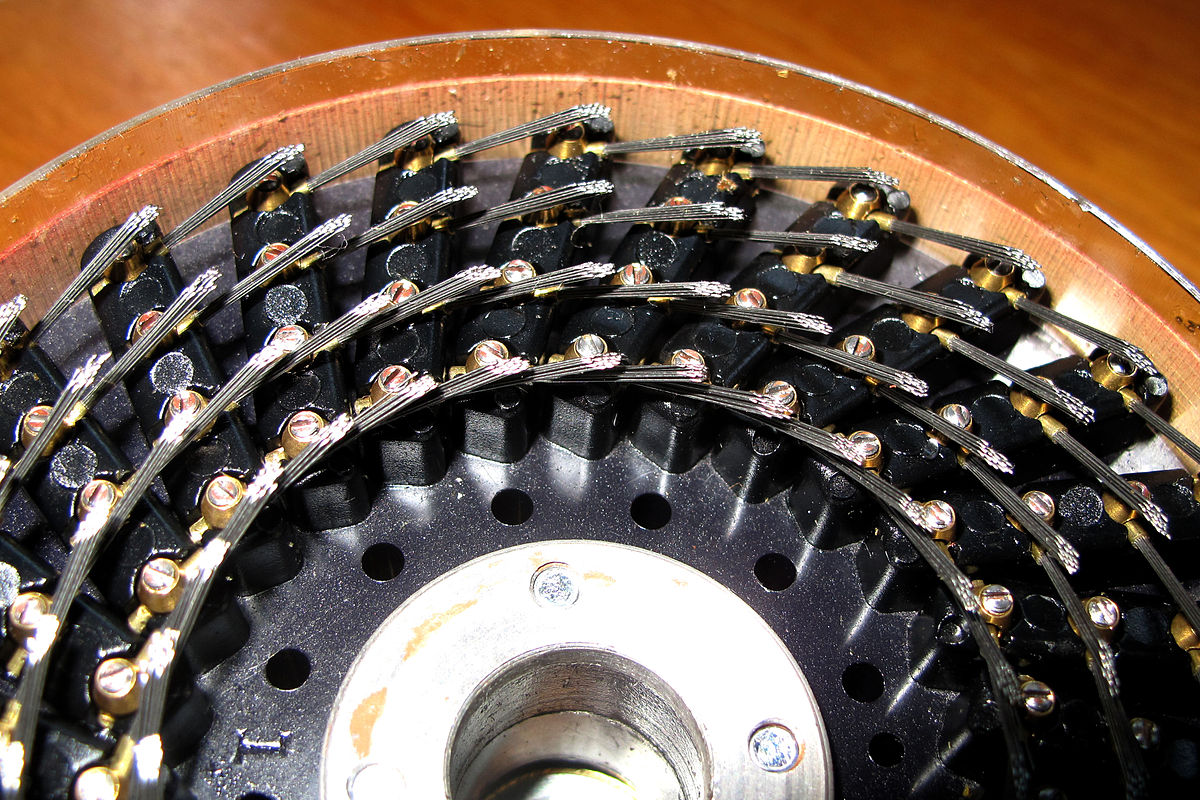
\includegraphics[width=0.4\linewidth]{Turing Bomb/WireBrushesOnBombeDrum}
	\caption{Die Kontakte der Scrambler\autocite{wiki:bombescrambler}}
	\label{fig:scrambler}
\end{figure} 


Die meisten Bomben bestanden aus dreimal zwölf Scramblersätzen.
Zwölf Scramblersätze ergeben eine \glqq Chain\grqq.
Ein Scramblersatz bestand aus drei Scrambler und simulierte eine Enigma-Maschine.
Der Grund, warum zwölf \glqq Enigmas\grqq{} parallel verwendet werden, ist, da somit eine komplette Ausgangsstellung der Walzen für das jeweilige Crib in einem Arbeitsgang überprüft werden kann.
Der unterste Scrambler eines Scramblersatzes repräsentiert die rechte, schnelle Walze einer Enigma-Maschine.
Der mittlere und oberste Scrambler ist repräsentativ für die mittlere und linke Walze der Enigma-Maschine.
Da die Scrambler keine Übertragskerbe besitzen, bewegt sich der nächste Scrambler immer nach einer vollen Rotation des aktuellen Scramblers, unabhängig von der Startposition.

Wurde nun durch die Mitarbeiter von Bletchley Park ein passendes Menü bestimmt, konnten die Scrambler in ihre Ausgangsstellung gebracht werden. 
Hierfür muss in dem Zyklus eine \glqq Route\grqq{} bestimmt werden.
Für den Zyklus in~\cref{fig:crib_cipher_cycle} könnte die Route lauten: \texttt{W $\to$ S $\to$ A $\to$ R $\to$ G $\to$ E $\to$ V $\to$ S}.

Die Zahlen auf den Kanten werden als \glqq Offsets\grqq{} für die untersten Walzen benutzt.
In unserem Beispiel sind also die Ausgangsstellungen der Scrambler also \texttt{AAA}, \texttt{AAL} und so weiter.
Sollen jetzt auch noch Ausleger, oder andere Tupel-Kombinationen wie 5 und 11 eingebunden werden, so können diese einfach an passender Stelle eingefügt werden: \texttt{AAD, AAE, AAK}.
Die Gesamtlänge der Elemente des Zyklus darf nicht zwölf überschreiten.

\subsection{Terminal}\label{subsec:terminal}
Auf der Rückseite der Bombe befinden sich dreimal 26 Terminal-Kontakte.
Ein 26er-Terminal-Satz ist jeweils einer Chain zugeordnet.
Jeder Kontakt in einem Terminal-Satz repräsentiert jeweils einen Buchstaben im Alphabet.
Jeder der 26 Kontakte hat 26 kleinere Kontakte, die wieder das Alphabet repräsentieren.
Wird nun im \emph{A}-Terminal an den \emph{e}-Kontakt Spannung angelegt, so wird die Hypothese getestet, dass der Geheimtext mit der Steckerbrett-Verbindung $A \Leftrightarrow E$ verschlüsselt wurde.

\subsection{In und Outs}\label{subsec:in_und_out}
Auf der Rückseite befinden sich Kontakte, die mit \glqq In\grqq{} und \glqq Out\grqq{} gekennzeichnet sind.
Wieder drei mal zwölf In- und Out-Paare, jeweils für die Scramblersätze.
Nun werden die Terminals mit den In und Outs verbunden.
Da der gewählte Routen-Startpunkt bei \glqq W\grqq{} liegt, wird der erste Scramblersatz auf das Offset \texttt{AAA} eingestellt.
Darauf wird das Terminal \emph{W} mit dem ersten In-Kontakt verbunden.
Der nächste Routen-Punkt \glqq S\grqq{} wird durch einen \glqq Brücken-Konnektor\grqq{} dem ersten Out mit dem zweiten In und dem Terminal \emph{S} verbunden.

\subsection{Diagonalbrett}\label{subsec:diagonalboard}
Gordon Welchman fiel auf, dass bei frühen Bomben nicht die Kommutativität des Steckerbretts beachtet wurde.
Ist $A$ mit $B$ gesteckert, so muss auch $B$ mit $A$ gesteckert sein.
Das Diagonalbrett stellte diese kommutativen Verbindungen her.
Für die Bombe heißt dies, dass wenn im \emph{A}-Terminal an den \emph{b}-Kontakt Spannung angelegt wird,
so auch der \emph{a}-Kontakt im \emph{B}-Terminal aktiv wird.
Dies trug maßgeblich zur Effizienz der Bombe bei.
Der Kontakt gleich dem Terminal-Buchstaben wird \glqq Self-Steckered\grqq{} genannt und stellt keine Steckerbrett-Verbindung dar.

\begin{figure}[htbp]
	\centering
%	\begin{tikzpicture}[scale=0.7, every node/.style={scale=0.8}]
%		\foreach \i in {0,..., 4}{
%			\foreach \j in {0,..., 4}{
%				\fill (\i*1.5, \j*1.5) circle (2pt); 
%			}
%			\draw (\i*1.5, \i*1.5) circle (4pt);
%
%		}
%		
%		\foreach \i in {1,...,4}{
%			\foreach \j in {1,...,4}{
%				\node[below] at (\i*1.5, \j*1.5) {\char\numexpr97+\i};			
%			}
%		}
%		
%		\foreach \i in {1,..., 4}{
%			\node[left] at (0, \i*1.5) {\char\numexpr65+\i};
%			\node[below] at (\i*1.5, 0) {\char\numexpr65+\i};
%		}
%		
%		\node[below left] at (0,0) {A};
%		
%		
%	\end{tikzpicture}
	\documentclass{standalone}
\usepackage{tikz}

\begin{document}
	\begin{tikzpicture}[scale=0.7, every node/.style={scale=0.8}]
		
		%Säulen
		\foreach \i in {0,2,4,6} {
			\foreach \j in {0,0.2,0.4,0.6} {
				\draw[thin] (\i+\j,1.5) -- (\i+\j,5+\j*2);
			}
			\node[below] at (\i+0.3, 1.5) {\emph{\char\numexpr65+\i/2}};
		}
		
		
		%Querverbindungen
		\foreach \j in {0.2,0.4,0.6} {
			\draw[thin](\j,5+\j*2) .. controls (\j*5,5+\j*1.5) .. (\j*10,5);
		}	
		
		\foreach \j in {0.4, 0.6} {
			\draw[thin](\j+2,5+\j*2) .. controls ({(\j + 2 + \j*10 + 0.2)/2},5+\j*1.6) .. (\j*10+0.2,5.4);
		}
		
		\draw[thin](4.6,6.2) .. controls (5.25,6.1) .. (6.4,5.8);
		
		%TODO at A terminal
		%		\draw[->] (-1,5.6) -- (0.2,5.4) node[left] at (-1,5.6) {\emph{b}-Kontakt im \emph{A}-Terminal};
	\end{tikzpicture}
\end{document}
	\caption{Diagonalbrett Verbindungen}
	\label{fig:diagonal_board_connections}
\end{figure}



\subsection{Commons}\label{subsec:commons}
Sollen nun auch noch Ausleger oder andere Graphen-Konstrukte miteinbezogen werden, reicht ein In- und Out-Kontakt nicht aus.
Hierfür gibt es dreimal sechs Common-Kontaktblöcke à fünf Kontakte.
Commons-Kontakte sind blockweise mit CO1, CO2 et cetera gekennzeichnet.
Sechs Blöcke sind einer Chain zugeordnet.
Die Kontakte eines Blocks sind miteinander verbunden.
Somit ist es möglich, den Out-Kontakt des Scramblersatzes, der dem \glqq E\grqq{} in unserem Zyklus entspricht, mit Terminal \emph{V} und \emph{N} und den jeweiligen Ins der Scramblersätze zu verbinden.
In~\cref{fig:bombe_rear} sind die Terminals, Commons und In und Outs mit den \glqq Brücken-Konnektoren\grqq{} zu sehen.
\nopagebreak
\begin{figure}[htbp]
	\centering
	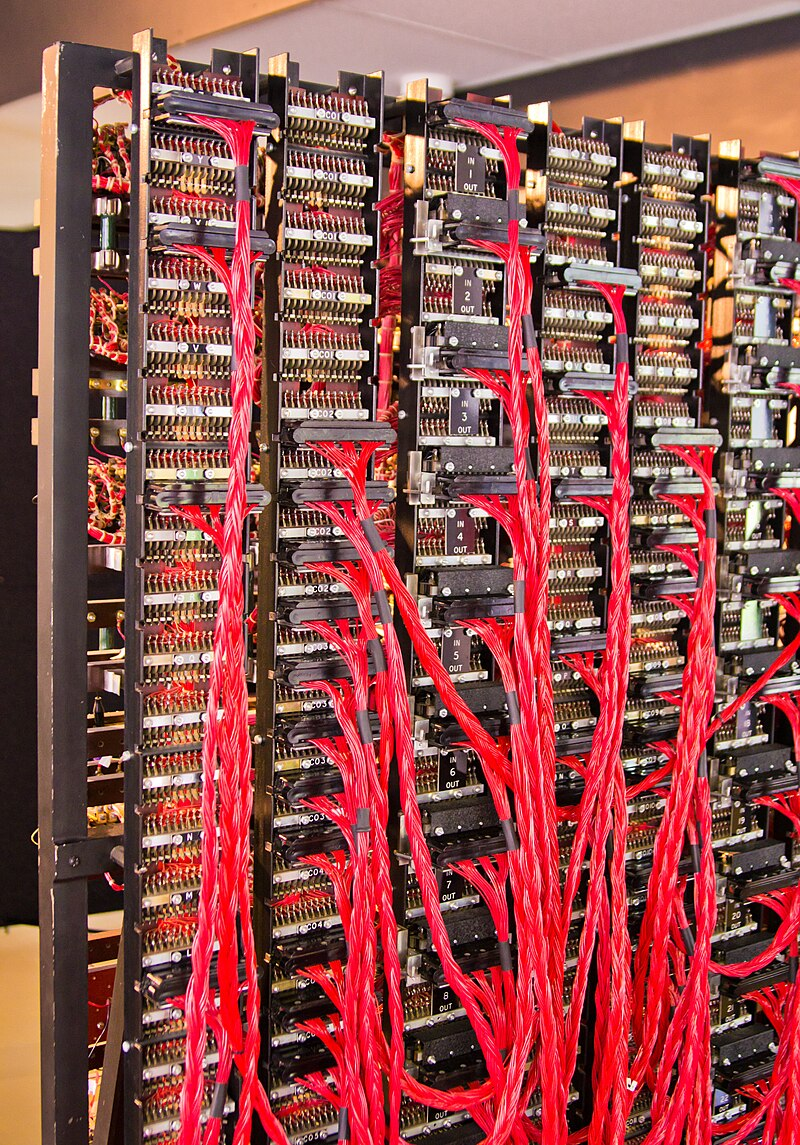
\includegraphics[width=0.5\linewidth, clip, trim=2cm 25cm 5cm 2cm]{Turing Bomb/Bletchley_Park_Bombe_Rear}
	\caption{Rückansicht der Bombe\autocite{wiki:bomberear}}
	\label{fig:bombe_rear}
\end{figure}

\subsection{Test-Register}\label{subsec:test-register}
Um eine Steckerbrett-Verbindungs Hypothese zu testen, muss ein Test-Register bestimmt werden.
Dies sollte ein Buchstabe im Menü sein, der sehr viele Verbindungen hat.
In dem Fall von~\cref{fig:crib_cipher_cycle} wäre der Buchstabe \glqq G\grqq{} geeignet.
Nun muss ein Test-Buchstabe bestimmt werden.
Fällt die Wahl zum Beispiel auf \emph{A}, so wird die Hypothese der Steckerbrett-Verbindung $A \Leftrightarrow G$ getestet.
Es wird vermutet, dass während des Chiffrierungs-Prozesses die Steckerbrett-Verbindung $A \Leftrightarrow G$ benutzt wurde.

\begin{figure}[htbp]
	\centering
	\documentclass{standalone}
\usepackage{tikz}

\begin{document}
	\begin{tikzpicture}[scale=0.7, every node/.style={scale=0.8}]
		%Säulen
		\foreach \i in {0,2,4,6} {
			\foreach \j in {0,0.1,0.2,0.3} {
				\draw[thin] (\i+\j,1) -- (\i+\j,5+\j*2);
			}
			\node[below] at (\i+0.15, 1) {\emph{\char\numexpr65+\i/2}};
		}
		%		\draw[very thick] (2.2,1) -- (2.2,5.4);
		
		%		\draw[thin](0,9) .. controls (1,9.05) .. (2,9);
		
		%Querverbindungen
		\foreach \j in {0.1,0.2,0.3} {
			\draw[thin](\j,5+\j*2) .. controls (\j*10,5+\j*1.5) .. (\j*20,5);
		}	
		\draw[very thick] (0.1,1) -- (0.1,5.2) .. controls (1,5 + 0.1 * 1.5) .. (2,5) -- (2, 1);
		
		\foreach \j in {0.2, 0.3} {
			\draw[thin](\j+2,5+\j*2) .. controls ({(\j + 2 + \j*20 + 0.1)/2}, 5+\j*1.5) .. (\j*20 + 0.1, 5.2);
		}
		
		
		\draw[thin](4.3,5.6) .. controls (5.25,5.5) .. (6.2,5.4);
		
		\foreach \j in {0,0.1,0.2,0.3} {
			\draw[thin] (2+\j,2+\j) -- (4+\j,2+\j);
			\fill (2+\j,2+\j) circle (1pt);
			\fill (4+\j,2+\j) circle (1pt);
		}
		\fill (2.8, 1.9) rectangle (3.5, 2.4);
		\node[above] at (3.2, 2.4) {\texttt{1: AAA}};
		
		\foreach \j in {0,0.1,0.2,0.3}{
			\draw[thin] (\j, 3+\j) -- (4+\j, 3+\j);
			\fill (\j,3+\j) circle (1pt);
			\fill (4+\j,3+\j) circle (1pt);
		}
		
		\fill (0.8, 2.9) rectangle (1.5, 3.4);
		
		\node[above] at (1.2, 3.4) {\texttt{2: AAB}};
	\end{tikzpicture}
\end{document}
	\caption{Diagonalbrett Verbindungen mit Scrambler Verbindungen}
	\label{fig:diagonal_board_connections_w_scrambler}
\end{figure}

In~\cref{fig:diagonal_board_connections_w_scrambler} wird die Hypothese der Steckerbrett-Verbindung $A \Leftrightarrow B$ getestet.
Unser Test-Register ist \emph{A}.
Es wurde ein Scramblersatz mit der Grundstellung \texttt{AAA} konfiguriert und Terminal \emph{B} mit dem ersten In und Terminal \emph{C} mit dem ersten Out verbunden.
Ein weiterer Scramblersatz wurde auf die Grundstellung \texttt{AAB} konfiguriert und dem zweiten In mit dem ersten Out, welcher durch den Brücken-Konnektor auch mit Terminal \emph{C} verbunden ist, verbunden.
Außerdem wurde das zweiten Out mit Terminal \emph{A} verbunden.
Die Tupel in~\cref{fig:diagonal_board_connections_w_scrambler} sind \texttt{B:C} an erster und \texttt{C:A} an zweiter Stelle. 
Da das Steckerbrett keinen Einfluss auf den Verlauf des Zyklus hat, spielt es keine Rolle, welche Hypothese getestet wird.
%Der Zyklus-Verlauf für~\cref{fig:diagonal_board_connections_w_scrambler} ist B $\rightarrow$ C $\rightarrow$ A\textellipsis.
Nun wird \emph{a} durch den Scramblersatz permutiert.
Ergibt sich durch die Permutation von \emph{a} ein anderer Buchstabe als \emph{c}, müsste die Steckerbrett-Verbindung signalisiert durch den aktiven Kontakt während der Chiffrierung benutzt worden sein.

Die Bombe hält in zwei Fällen:
\begin{enumerate}
	\item In dem Test-Register ist nach den Permutationen ein Kontakt aktiv – die Hypothese hat sich bewahrheitet.
	\item In dem Test-Register sind nach den Permutationen 25 Kontakte aktiv – die Hypothese ist falsch, aber die nicht aktiven Kontakte in den Terminals geben die \glqq richtige\grqq{} Steckerbrett-Verbindung an. (Reductio ad absurdum)
\end{enumerate}

Die anderen Fälle werden von der Bombe ignoriert.
Angenommen unser erster Scramblersatz permutiert das \emph{a} im \emph{B}-Terminal zu einem \emph{c} und unser zweiter Scramblersatz permutiert dieses \emph{c} zu einem \emph{d} im \emph{A}-Terminal, so erzeugt dies ein Widerspruch.
Es wurde die Hypothese der Steckerbrett-Verbindung $A \Leftrightarrow B$ aufgestellt, aber damit der dritte Buchstabe im Zyklus bei der aktuellen Walzenlage einem \emph{a} entsprechen kann, muss zusätzlich $A \Leftrightarrow D$ herrschen.
Dies ist eine widersprüchliche Aussage, da Buchstaben nur mit einem anderen verbunden sein können –- die Walzen rotieren.

Die Tupel-Kombinationen 5 und 11 in~\cref{fig:crib_cipher_cycle} sind besonders effektiv, da sich die Anzahl der aktiven Verbindungen rasch \glqq aufschaukelt\grqq.



	
	\chapter{Implementierung der Turing-Welchman-Bombe}\label{ch:impl_bombe}
%\section{Enigma-Maschine}\label{sec:impl_enigma}
%Um die Bombe in Software Nachzubilden, muss zuerst eine Enigma-Maschine nachgebildet werden.
%\subsection{Rotoren}\label{subsec:impl_enigma_rotor}
%Die Verdrahtung der Rotoren wurden als Vektor realisiert.
%Der zu permutierende Buchstabe wird hierfür als Index in den Vektor genutzt.


\section{Menü Algorithmus}\label{sec:cycle-finding-algorithm}
Um eine Turing-Welchman-Bombe in der Programmiersprache C nachzubilden, muss zuerst ein Algorithmus entworfen werden, welcher das Menü durch ein von dem Nutzer vorgegebenes Crib und 
%TODO
Geheimtext bildet.

Hierfür werden die einzelnen Buchstaben als Knoten mithilfe einer Struktur dargestellt, welche zum einen den Buchstaben und zum anderen einen Vektor mit den anliegenden Auslegern beinhaltet.
Die Buchstaben-Tupel wurden ebenfalls als Struktur dargestellt, welche zwei Knoten, die Position im Crib und einen Booleschen Wert beinhaltet, welcher aussagt, ob dieses Tupel zum Zyklus beiträgt.


\noindent
\lstinputlisting[style=mystyle, caption={Realisierung der Menü Strukturen}, label={lst:code_impl_menu}]{Implementierung/menu_structs.c}
Die Tupel werden nun in einer \glqq Nachschlagetabelle\grqq{} abgelegt.
Diese Tabelle hat 26 Stellen, repräsentativ für das Alphabet.
Ein jeweiliges Tupel wird sowohl unter dem ersten als auch unter dem zweiten Buchstaben abgelegt. 
Tupel wie \texttt{W:S} werden also unter \texttt{W} und unter \texttt{S} abgelegt.
Ein Tiefensuche-Algorithmus, der modifiziert wurde, um weniger \glqq gierig\grqq{} zu agieren, schlägt die Tupel in der Tabelle nach und markiert die besuchten Tupel.
%Bei dem Rücksetzverfahren der Tiefensuche wird die Markierung der Tupel, die nicht zum Zyklus beitragen entfernt.
Das Ergebnis ist eine gemessene, lineare Laufzeit.\footnote{Es wurden Crib-Längen bis 26 betrachtet, um zu garantieren, dass die lineare Laufzeit bei einer maximalen Länge von 13 Buchstaben gegeben ist.
Der Laufzeit-Graph ist im Anhang enthalten:~\cref{fig:app_menu_runtime}}

Das Menü wird als Vektor von \texttt{CribCipherTuple} in einer Struktur mit der Länge abgelegt.
Da es erforderlich ist, eine eindeutige \glqq Route\grqq{} durch das Menü anzugeben, werden Tupel-Kombinationen bei den betroffenen Knoten als Ausleger angegeben. 
Die Bombe kann somit im Falle der \glqq Scramblersatz-Knappheit\grqq{} entscheiden, ob sie diesen (nicht notwendigen) Bestandteil des Menüs aufnehmen möchte.

\section{Modellierung der Turing-Welchman-Bombe}\label{sec:model}
\subsection{Scrambler}\label{subsec:impl_scrambler}
Wie in~\cref{subsec:vorbereitungen} erklärt, vernachlässigt die Bombe den Übertragzeitpunkt der Walzen.
Die Software-Implementation berücksichtigt ebenfalls die Übertragskerbe der Rotoren nicht.
%TODO Enigma Software gegeben erwähnen?
Die Verdrahtung der Scrambler wird als Vektor abgebildet, welcher wie in~\cref{fig:rot1_wiring} die Permutation für jeden Buchstaben speichert.
Die Buchstaben werden jedoch nicht in der typischen ASCII-Kodierung gespeichert, sondern auf den Wertebereich 0--25 abgebildet.
Mit dem Resultat kann somit direkt der Vektor des nächsten Scramblers indiziert werden.
Es muss zudem die Walzenlage mitgeführt werden, welche mit dem zu permutierenden Buchstaben addiert wird, um den Vektor-Index zu bilden.
Der Wertebereich wird durch eine Modulo-Operation zwischen 0 und 25 gehalten.

\subsection{Terminal}\label{subsec:impl_terminal}
Die Kontakte der Terminals werden als Struktur dargestellt.
Es beinhaltet einen 32-Bit-Integer, welcher als Bitvektor mit 26 seiner Stellen die aktiven Kontakte repräsentiert.
Die Anzahl der aktiven Kontakte wird ebenfalls als Integer mitgeführt.
Da es in Bezug auf die Laufzeit medioker ist, alle 26 Stellen des Bitvektors traversieren zu müssen, um zu überprüfen, welche der 26 Kontakte aktiv sind, wurde ein normaler Vektor eingeführt, der die aktiven Kontakte \glqq dicht\grqq{} speichert.
%TODO Artikel vor Nummer
Zuletzt wird der Buchstabe/die Nummer des jeweiligen Kontakts in der Struktur gespeichert.

\noindent
\lstinputlisting[style=mystyle, caption={Realisierung der Terminals}, label={lst:code_impl_terminal}]{Implementierung/terminal.c}

Permutiert ein Scrambler einen Buchstaben, wird mithilfe des Bitvektors überprüft, ob dieser Kontakt bereits aktiv ist.

Hierbei gibt es zwei Szenarien:
\begin{enumerate}
	\item Der Kontakt ist inaktiv: In dem Bitvektor wird die repräsentative Stelle aktiviert, der Buchstabe wird in dem normalen Integer Vektor abgelegt und die Anzahl der aktiven Verbindungen inkrementiert.
	
	\item Der Kontakt ist aktiv: Dieser Buchstabe wird ignoriert. 
\end{enumerate}

Die Terminal-Struktur beinhaltet einen Vektor mit 26 Kontakte und einen Zeiger auf den Kontakt des Test-Registers.
Bei dem Test-Register wird hierbei nicht von einem \glqq normalen\grqq{} Kontakt unterschieden.

\subsection{In und Outs}\label{subsec:impl_in_und_outs}
Die In- und Out-Kontakte werden mit dem dazugehörigen Scramblersätzen als Knoten dargestellt.
Sämtliche Verbindungen durch Kabel und Brücken-Konnektoren des analogen Originals werden hier durch Zeiger auf Kontakte ersetzt, so auch die In- und Out-Kontakte.

\subsection{Diagonalbrett}\label{subsec:impl_diagonal_board}
Das Diagonalbrett als native Datenstruktur darzustellen, hat sich als ein eher schlechter Einfall herausgestellt.
Eine Möglichkeit das Verhalten mit einer Datenstruktur zu imitieren, ist es, die einzelnen Kontakte der Terminals als Vektor mit Zeiger auf Booleschen Werten abzubilden.
Hierbei zeigt zum Beispiel der \emph{a}-Kontakt des \emph{B}-Terminals und der \emph{b}-Kontakt des \emph{A}-Terminals auf den gleichen Booleschen Wert.
Somit ist die Verbindung $A \Leftrightarrow B$ abgebildet.
Jedoch wäre es hier abermals nötig, den gesamten Vektor zu traversieren, um die aktiven Kontakte herauszufinden.
Die entsprechenden Kontakte müssten nun wieder einen normalen Vektor besitzen, in dem die aktiven Kontakte \glqq dicht\grqq{} stehen, damit die Scrambler effektiv arbeiten können.
Somit wäre es hier abermals notwendig die Kontakte separat zu behandeln.

Aus diesem Grund wurde die Funktion des Diagonalbrettes in einer Funktion gekapselt:

\noindent
\lstinputlisting[style=mystyle, caption={Realisierung des Diagonalbrettes}, label={lst:code_impl_diag_board}]{Implementierung/diag_method.c}
%TODO TuringBombe Struct erklären?
Diese Funktion erhält drei Argumente: Einen Zeiger auf eine \texttt{TuringBombe} und zwei Integer, repräsentativ für die zwei Terminal-Buchstaben, die aktiviert werden sollen.


\subsection{Commons}\label{subsec:impl_commons}
Aufgrund der Einfachheit wurden die Commons in dieser Software-Implementation \glqq weg abstrahiert\grqq.
Diese wurden durch Zeiger auf den gleichen Kontakt ersetzt.
Die Anzahl der Kontakte pro Commons und die Gesamtzahl der verwendeten Commons wurde gezählt, sodass diese nicht die Anzahl des analogen Originals überschreiten.

\section{Algorithmus der Implementation}\label{sec:algorithm_bombe}
Im Gegensatz zur \glqq echten\grqq{} Bombe, welche eine Steckerbrett-Hypothese für die jeweils 17576 Walzenstellungen einer Walzenlage testet, testet die Software-Nachbildung eine Hypothese für alle Walzenstellungen der 60 möglichen Walzenlagen.
Eine modifizierte Breitensuche traversiert die Knoten des aufgespannten Graphen der \glqq Scrambler-Knoten\grqq.
Da es aufgrund der Tupel-Kombinationen nicht genügt, einige Knoten nur einmal zu besuchen, und das Diagonalbrett es schwierig macht, die Datenstruktur der Knoten linear zu durchlaufen, wird erneut eine \glqq Nachschlagetabelle\grqq{} benötigt.
Die Nachschlagetabelle besitzt 26 Stellen, jeweils für die 26 Terminal-Kontakte.
Die Knoten, die durch den In-Kontakt mit einem jeweiligen Terminal verbunden sind, werden in dieser Tabelle abgelegt.
Zuerst werden alle Scrambler-Knoten, die durch den In-Kontakt mit dem Test-Register verbunden sind, in die Warteschlange eingereiht. 
Danach werden die Commons der jeweiligen Knoten eingereiht und als Letztes die Knoten, welche an jene Kontakte anliegen, die durch direkte Permutation der Scrambler oder durch das Diagonalbrett aktiviert wurden.
Wird durch die Permutation eines Scramblers in dem mit ihm verbundenen Out-Kontakt kein neuer Kontakt aktiv, so werden die Knoten, welche durch den In-Kontakt mit dem jeweiligen Kontakt verbunden sind, nicht eingereiht.
%wird dieser Knoten als \glqq besucht\grqq{} gekennzeichnet und nicht mehr in die Warteschlange eingereiht.
Ist die Warteschlange leer, ergo keine Permutationen mehr möglich, wird das Test-Register überprüft.
%sind alle Permutationen abgeschlossen und das Test-Register wird überprüft.
Ergeben die Permutationen keine gültige Konfiguration, werden alle Kontakte die durch Permutation oder Diagonalbrett aktiviert wurden, deaktiviert. 
%und Knoten als nicht besucht gekennzeichnet.
Die Software-Nachbildung hält nach den in~\cref{subsec:test-register} beschriebenen Regeln.
%In Pseudocode könnte man den Algorithmus der Bombe so darstellen:
%\begin{algorithm}[htbp]
%	\caption{Bombe Algorithmus}
%	\begin{algorithmic}
%			\Procedure{Bombe}{$p_0 \dots p_{n-1} :$ [Char], $c_0 \dots c_{n-1} :$ [Char]}
%			\ForAll{\textsl{rotors} $\in$ \textbf{permut(rotor order)}, \textsl{pos} $\in$ \textbf{[AAA $\dots$ ZZZ]}}
%			\State plugs: Char $\rightarrow \{ $Char$\}$
%			\State plugs$(p_0)\ \cup= \{\textbf{'A'}\}$
%			\While{\textsl{plugs} changing}
%			\ForAll{\textsl{i} $\in$ \textbf{[0\dots n--1]}}
%			\State plugs($c_i$) $\cup=$ $\bigcup_{p \in \text{plugs}(p_i)}$ encrypt(\textsl{rotors, p, pos}+\textsl{i})
%			\State plugs($p_i$) $\cup=$ $\bigcup_{p \in \text{plugs}(c_i)}$ encrypt(\textsl{rotors, p, pos}+\textsl{i})
%			\EndFor
%			\EndWhile
%			\If{$\forall$ \textsl{S} $\in$ \textbf{cod(plugs)}: \#S < \#Char}
%			\State report(\textsl{pos, plugs})
%			\EndIf
%			\EndFor
%			\EndProcedure
%		\end{algorithmic}
%	\label{alg:algorithm}
%\end{algorithm}

	
%	\chapter{Häufigkeitsanalyse}\label{ch:haufigkeitsanalyse}
%	\section{Koinzidenzindex}\label{sec:koinzidenzindex}
%	\thispagestyle{scrheadings}
%	
%	Zunächst benötigen wir ein geeignetes Maß, um den Grad der Annäherung eines teilweise dechiffrierten Klartextes an authentisches Deutsch abzuschätzen.
%	Dafür verwenden wir den Koinzidenzindex:
%	
%	\fmbox{\textbf{Koinzidenzindex}\[IC = \frac{\sum_{i=A}^{Z}f_i(f_i-1)}{N(N-1)}\]}
%	
%	
%	Sei $f_i$ die Häufigkeit des Buchstabens in Abhängigkeit von $i$ und $N$ die Gesamtanzahl der Buchstaben.
%	Wir Summieren also die Anzahl der Buchstabenpaare auf, und teilen diese durch die Anzahl der allgemein möglichen Buchstabenpaare.
%	Der Koinzidenzindex ist also ein Maß für die Buchstabenverteilung.
%	Für ein Text bestehend aus zufälligen Buchstaben beträgt der $IC \approx$ 0.038; wobei er für Deutsch $\approx$ 0.076 beträgt.
	
	
	\newpage
	\chapter{Glossar}\label{sec:glossar}
	\begin{itemize}
		\item Blechley-Park: Zentrale militärische Dienststelle, die sich im Zweiten Weltkrieg erfolgreich mit der Entzifferung des deutschen Nachrichtenverkehrs befasste.
		\item Crib: Klartextfragment, welches an einer bestimmten Stelle im Geheimtext vermutet wurde.
		\item $D_K$: Die Dechiffrierfunktion.
		\item $E_K$: Die Chiffrierfunktion.
		\item Gardening: Das Provozieren von Funksprüchen, welche einen bestimmten Klartext enthalten.
		\item Menü: Ein Graph aus Crib-Geheimtext Tupeln, der die Einstellungen der Bombe vorgibt.
		\item Involution: Eine selbstinverse Abbildung.
		\item Schlüssler: Person, die Nachrichten ver- oder entschlüsselt.
		\item Spruchkopf: Unverschlüsselter, erster Teil einer Nachricht, welcher die Uhrzeit, die Buchstabenanzahl, die Grundstellung und den verschlüsselten Spruchschlüssel beinhaltete.
		\item Spruchschlüssel:  Individueller Schlüssel für einen Funkspruch.
	\end{itemize}
	
	\chapter{Quellen}\label{ch:sources}
	\section{Einzelnachweise}\label{sec:einzelnachweise}
	\printbibliography[keyword=sources, heading=none, title={}]
	\section{Bildnachweise}\label{sec:bildnachweise}
	\printbibliography[keyword=pictures, heading=none, title={}]
	\nocite{*}
	\thispagestyle{plain}
	
	
	\appendix
	\chapter{Anhang}\label{ch:appendix}
\section{Übertragung der Nachrichten}\label{sec:msg-trans}

\vspace{1cm}
\begin{samepage}
	\thispagestyle{empty}
	\begin{figure}[htbp]
		\centering
		\scalebox{\scalepic}{
			\begin{tikzpicture}
				\tikzset{func/.style={rectangle, draw, fill=func-red, rounded corners}}
				\tikzset{arr/.style={-{Stealth[scale=1]}, thick, shorten <=.1cm, shorten >=.1cm}}
				\tikzset{think/.style={cloud callout, callout relative pointer={(0.2, -0.8)}, cloud puff arc=120, aspect=1.5, align=center, fill=white, draw}}
				
				\node at +(0,.5cm) (alice){};
				\node[think, above=1.8cm of alice] {$K_S$};
				\Strichmaxerl[5] 
				\node[below] at (-0.3, 0) {Alice};
				\node[func, right=of alice] at +(0, .5cm) (enigma) {Enigma};
				\draw[arr] (alice) -- node[above] {$K_S$} (enigma);
				\draw[arr] (enigma.north)+(0, .7cm) node[above] {$K_T$} -- (enigma);
				\node[right=2cm of enigma] (dest) {};
				\draw[arr] (enigma.east) -- node[above] {$K_S'$} (dest);
				\draw[gray] 
				(dest)++(0,-0.2cm)
				-- ++(0,0.5cm) 
				-- ++(2cm,0) 
				-- ++(0,-0.5cm) 
				-- ++(-0.5cm, 0.1cm) 
				-- ++(-0.5cm, -0.1cm) 
				node[above=.1cm, black] {\tiny Spruchkopf}
				-- ++(-0.5cm, 0.2cm) 
				-- ++(-0.5cm, -0.2cm)
				-- cycle;
 				\draw[arr] ($(enigma.north)+(.3cm, 1cm)$) -| ($(dest)+(1cm, .3cm)$);
			\end{tikzpicture}
		}
		\caption{Erzeugung Spruchkopf}
		\label{fig:msg-head}
	\end{figure}
	\begin{figure}[htbp]
		\centering
		\scalebox{\scalepic}{
			\begin{tikzpicture}
				\tikzset{func/.style={rectangle, draw, fill=func-red, rounded corners}}
				\tikzset{arr/.style={-{Stealth[scale=1]}, thick, shorten <=.1cm, shorten >=.1cm}}
				\node at +(0,.5cm) (alice){};
				\Strichmaxerl[5] 
				\node[below] at (-0.3, 0) {Alice};
				\node[func, right=of alice] (enigma) {Enigma};
				\draw[arr] (alice) -- node[above] {$M$} (enigma);
				\draw[arr] (enigma.north)+(0, .7cm) node[above] {$K_S$} -- (enigma);
				\node[right=of enigma] (dest) {};
				\draw[arr] (enigma.east) -- node[above] {$M^\prime$}(dest);
				\draw[gray] 
				(dest)++(0,0.2cm) 
				-- ++(0,-1cm) 
				-- ++(2cm,0)
				-- ++(0,1cm)
				-- ++(-0.5cm, 0.1cm) 
				-- ++(-0.5cm, -0.1cm) 
				-- ++(-0.5cm, 0.2cm) 
				-- ++(-0.5cm, -0.2cm)
				-- cycle; 
			\end{tikzpicture}
		}
		\caption{Chiffrierung Nachricht}
		\label{fig:enc-msg}
	\end{figure}
	\begin{figure}[htbp]
		\centering
		\scalebox{\scalepic}{
			\begin{tikzpicture}
				\tikzset{func/.style={rectangle, draw, fill=func-red, rounded corners}}
				\tikzset{arr/.style={-{Stealth[scale=1]}, thick, shorten <=.1cm, shorten >=.1cm}}
				
				\node at +(-0.3,.5cm) (bob){};
				\Strichmaxerl[5] 
				\node[below] at (-0.3, 0) {Bob};
				\node[func, left=of bob] (enigma) {Enigma};
				\draw[arr] (enigma) -- node[above] {$K_S$}(bob);
				\draw[arr] (enigma.north)+(0, .7cm) node (top env) {} -- node[right, midway] {$K_T$} (enigma);
				\draw[gray] 
				(top env)++(-1cm,0)
				-- ++(0,0.5cm) 
				-- ++(2cm,0) 
				-- ++(0,-0.5cm) 
				-- ++(-0.5cm, 0.1cm) 
				-- ++(-0.5cm, -0.1cm) 
				node[above=.1cm, black] {\tiny Spruchkopf}
				-- ++(-0.5cm, 0.2cm) 
				-- ++(-0.5cm, -0.2cm)
				-- cycle;
				\coordinate (top env start) at (enigma.north)+(-1cm, .7cm);
				\node[] at (top env start) (top env) {};
				
				\node[left=of enigma] (dest) {};
				\draw[arr] (dest) -- node[above] {$K_S^\prime$} (enigma);
				\node[left=1.7cm of dest] (bottom env) {};
				\draw[gray] 
				(bottom env)++(0,-0.2cm) 
				-- ++(0,0.5cm) 
				-- ++(2cm,0) 
				-- ++(0,-0.5cm) 
				-- ++(-0.5cm, 0.1cm) 
				-- ++(-0.5cm, -0.1cm) 
				node[above=.1cm, black] {\tiny Spruchkopf}
				-- ++(-0.5cm, 0.2cm) 
				-- ++(-0.5cm, -0.2cm)
				-- cycle;
			\end{tikzpicture}
		}
		\caption{Dechiffrierung Spruchschlüssel}
		\label{fig:dec-head}
	\end{figure}
	\begin{figure}[H]
		\centering
		\scalebox{\scalepic}{
			\begin{tikzpicture}
				\tikzset{func/.style={rectangle, draw, fill=func-red, rounded corners}}
				\tikzset{arr/.style={-{Stealth[scale=1]}, thick, shorten <=.1cm, shorten >=.1cm}}
				\node at +(-0.3,.5cm) (bob){};
				\Strichmaxerl[5] 
				\node[below] at (-0.3, 0) {Bob};
				\node[func, left=of bob] (enigma) {Enigma};
				\draw[arr] (enigma.north)+(0, 1cm) -- node[right, midway] {$K_S$} (enigma);
				\draw[arr] (enigma) --  node[above] {$M$} (bob);
				\node[left=of enigma] (dest) {};
				\draw[arr] (dest) -- node[above] {$M^\prime$} (enigma);
				\node[left=1.7cm of dest] (bottom env) {};
				\draw[gray] 
				(bottom env)++(0,0.2cm) 
				-- ++(0,-1cm) 
				-- ++(2cm,0)
				-- ++(0,1cm)
				-- ++(-0.5cm, 0.1cm) 
				-- ++(-0.5cm, -0.1cm) 
				-- ++(-0.5cm, 0.2cm) 
				-- ++(-0.5cm, -0.2cm)
				-- cycle; 
			\end{tikzpicture}
		}
		\caption{Dechiffrierung Nachricht}
		\label{fig:dec-msg}
	\end{figure}
\end{samepage}

\section{Laufzeit Menü Algorithmus}\label{sec:runtime_menu}
\begin{figure}[htbp]
	\centering
	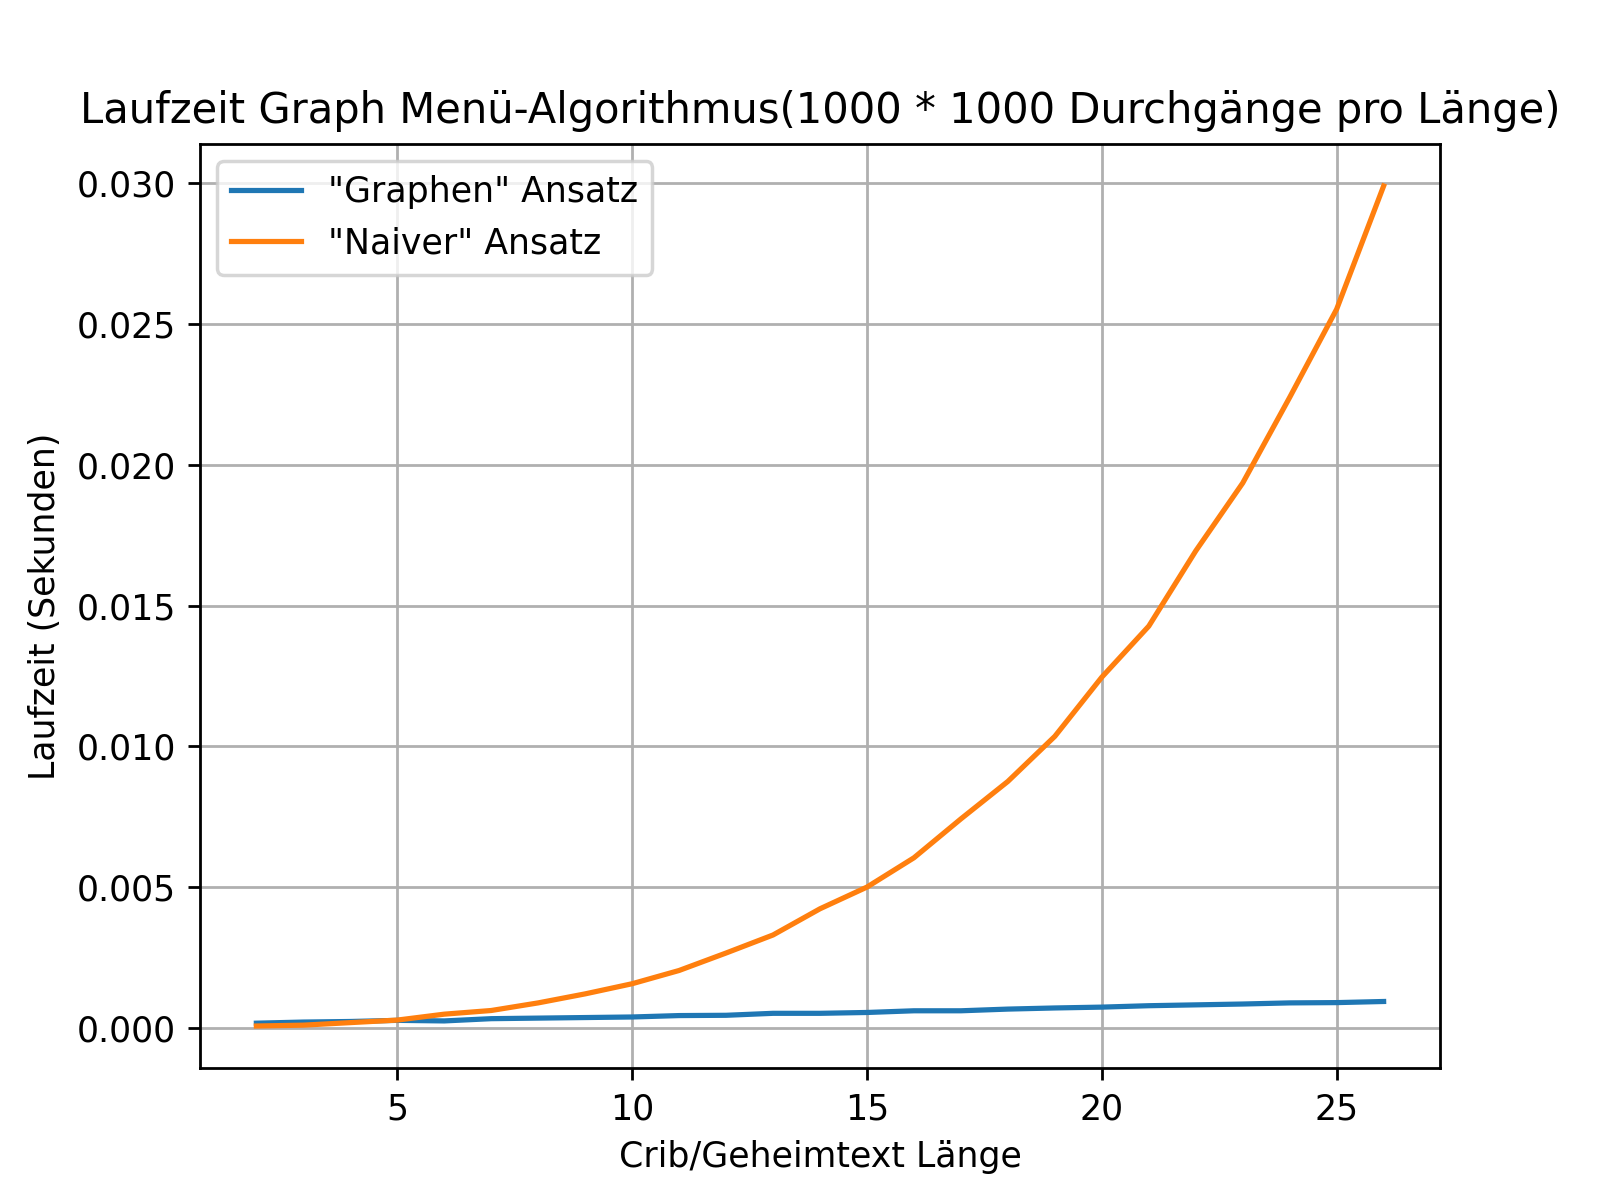
\includegraphics[width=.7\linewidth]{Turing Bomb/Crib-Cipher Loop/Runtime Graph Graph vs Force}
	\caption{Laufzeit-Graph Menü-Algorithmus}
	\label{fig:app_menu_runtime}
\end{figure}
Es wurden pro Länge 1000 Zufalls Crib und Geheimtexte generiert und diese
jeweils mit 1000 Durchgängen getestet.
\end{document}
